%!TEX root = ../thesis_a4.tex

\chapter[An enhancement: class-based tag recommendation][An enhancement: class-based tag rec.]{An enhancement: class-based tag recommendation}
\label{sec:class}

\section{Introduction}
\label{sec:class:introduction}

%Free-form semantically-meaningful textual labels, called tags, are extensively used in online sharing platforms for describing and annotating contents. Systems that provide the functionality for making these annotations are normally referred to as collaborative tagging systems. Several problems arise when users annotate shared and/or online resources~\citep{halpin2006}. The most typical ones are tag scarcity, the use of different tags to refer to a single concept (synonymy), the ambiguity in the meaning of certain tags (polysemy), the commonness of typographical errors, the use of user-specific naming conventions, or the use of different languages. To minimise some of these problems, tag recommendation systems can be employed to suggest potentially relevant tags during the annotation process~\citep{jaske2007}. As users are exposed to the suggestions of the system, the annotation process partially shifts from the creation of textual labels to the recognition of tags in a list~\citep{Sood2007}, and thus all users receive a certain common influence from the system. Hence, tag recommendation serves the purpose of consolidating the vocabulary of collaborative tagging systems~\citep{Jaschke2009}.

%In general, tag recommendations are either based on content analysis of online resources or in the other tags that users introduce during the annotation process. In the case of content-based recommendations, a typical approach consists in, given a resource to be described, defining a neighbourhood of other resources (based on some similarity measure) and then recommending tags that are used to annotate resources in this neighbourhood~\citep{ivanov2010, moha2012}. Another approach is the use of machine learning techniques to learn mappings between tags and content features~\citep{Li2006, turnbull2008, Toderici2010}. On the other side, there are tag recommendation strategies which are based on the tags that users introduce during the annotation process itself, prior to the moment of the recommendation. 
%Disadvantages of these strategies compared to content-based recommendation methods are that they require the existence of at least one tag to provide recommendations, whereas content-based recommendation systems can provide recommendations to resources with no associated tags or other metadata.
%Nevertheless, tag recommendation methods based on the tags that users introduce during the annotation process have the advantage of not requiring any specific processing of the content of the resources being annotated, thus being typically less expensive in terms of computation resources and being more easily generalisable to other multimedia domains.
%These methods usually consider the \emph{folksonomy} (i.e.,~the set of associations between tags, users and content resources) of a collaborative tagging system to estimate tag similarity from their resource co-occurrence. In this way, candidate tags can be selected according to their similarity to the introduced tags, and a sorting algorithm can rank them in terms of estimated relevance~\citep{jaske2007, Sigurbjornsson2008, Garg2008, DeMeo2009}. In previous work, we described and evaluated a general scheme for folksonomy-based tag recommendation in collaborative tagging systems~\citep{Font2013}. Out of that scheme, eight particular methods were proposed which form the basis of the method presented in this work.

%Besides content-based and folksonomy-based tag recommendation systems, other approaches have been described in the literature. Anderson et~al.~\citep{Anderson2008} describe a tag recommendation system for Flickr\footnote{\texttt{www.flickr.com}}, a well known photo sharing site, which combines both content-based recommendations (by training a predictive model that learns the mapping between tags and extracted content image features) with folksonomy-based recommendations (following an strategy very similar to~\citep{Sigurbjornsson2008}). Naaman and Nair\citep{Naaman2008} describe another tag recommendation system for Flickr, which takes advantage of the geolocation metadata attached to images and recommends tags that other users employed in close areas. Chen et~al.~\citep{Chen2010} describe a tag recommendation system for video resources which crawls the web for information about these videos and identifies keywords to recommend as tags.

%Although it is quite common to personalise tag recommendation systems to the tagging behaviour of particular users by promoting, for example, tags that users introduced in past annotations~\citep{jaske2007, Garg2008, Lipczak2008, Rendle2009, Marinho2009, Cao2009}, most of the current systems do not introduce direct user feedback in the evaluation loop. Thus recommendations are generally evaluated using traditional information retrieval approaches based on the comparison of tag rankings produced by different methods, or using precision and recall metrics computed after a tag prediction task~\citep{Garg2008, Lipczak2008, Rendle2009, Cao2009, Marinho2009, Font2013}. 
%To the best of our knowledge, only three studies perform some kind of user-based evaluation. Sigurbj\"{o}rnsson and Zwol~\cite{Sigurbjornsson2008} automatically generate tag recommendations for several images from a Flickr dataset and then ask users to rate, in a four-point scale, whether the recommendations are appropriate to a given image. 
%Similarly, De Meo et~al.~\cite{DeMeo2009} extend the annotations of Delicious' bookmarks\footnote{\texttt{www.delicious.com}} and then ask users to evaluate the relevance of every tag/resource association. 
%J\"{a}schke et~al.~\cite{Jaschke2009} perform a small evaluation based on a real-world scenario where users have to tag bookmarks in BibSonomy\footnote{\texttt{www.bibsonomy.org}}. Specifically, precision and recall metrics are computed by comparing tag recommendations performed to every bookmark and the final taglines that users introduced. Due to its subjectiveness and many different ways to be accomplished, tag recommendation is not an easy task to evaluate, and some advantages and disadvantages can be found in both user-based and information retrieval evaluation approaches~\citep{Garg2008}.
%However, there is a clear lack of user-based evaluation in previous work, and we believe that every recommendation system should be validated at some point using both evaluation strategies. Proper user feedback should be helpful not only to compare tag recommendation methods but also to better understand the nature of the task and learn how can systems be improved.

In this chapter we build on the tag recommendation methods described in the previous chapter and extend them. Furthermore, we perform an evaluation of the extended recommendation system through an online experiment with real users. Hence, the contribution of the present chapter is twofold. 
Firstly, we propose an extended version of the best performing tag recommendation method described in Chapter~\ref{sec:general} (RankP@$\percentageOfPercentageStrategy$). The main idea behind this extended method is to exploit the automatic classification of the resources to be annotated into a number of predefined classes to further adapt the tag suggestions to the context of these classes. This classification is based on the tags that users start introducing during the annotation process. In this way, instead of personalising recommendations for particular users, we ``personalise'' them to particular classes of resources, and the extended tag recommendation system incorporates some domain-specific knowledge in the form of resource categories.
We evaluate the automatic classification process separately from the rest of the tag recommendation system.

Secondly, we perform a comprehensive user-based evaluation through an online experiment. In it, participants are presented with some resources which have to be annotated with the help of the tag recommendation system. 
These kinds of user-based evaluations are very costly, and we have seen that they are not very common in the tag recommendation literature (Sec.~\ref{sec:soa:evluation_of_tag_recommendation}). In our evaluation, we compare the recommendation method we proposed in previous work and the extended version we describe here along with two random baselines. Moreover, we perform a complementary evaluation based on a tag prediction task such as the one described in the previous chapter (Sec.~\ref{sec:general:evaluation_methodology}, also see Sec.~\ref{sec:soa:evluation_of_tag_recommendation}). 
%In Chapter~\ref{sec:general}, we evaluated our proposed tag recommendation methods through a tag prediction task, and compared them favourably against four baselines and two state of the art methods~\citep{Sigurbjornsson2008,Garg2008}. For this comparison, we used data from the folksonomies of Freesound and Flickr. Therefore, the recommendation methods were tested in the audio and image domains. Similar results were obtained in both scenarios.
In the previous chapter, we evaluated the tag recommendation methods in the audio and image domains (i.e.,~using data from Freesound and Flickr), and obtained similar results in both scenarios. In this chapter, due to the extended recommendation method being based on the automatic classification of resources, evaluations are solely carried out in the context of Freesound. 

%Results show that the newly proposed recommendation method brings a statistically significant improvement over the previous method, according to both user-based and prediction-based evaluations. Analysing user-based evaluation results we find that participants which are experienced in working with sound libraries tend to better appreciate the improvements of the new tag recommendation method. Moreover, we see that the more familiarised the users are with Freesound, the more the number of tag suggestions they accept as valid annotations. User feedback reveals that tag recommendation methods tend to be more useful when recommending broad tags (i.e.,~referring to generic concepts). Participants also recognise sound annotation as a particularly difficult task, specially if the resources being annotated are not authored by themselves.

The rest of this chapter is organised as follows. 
First, in Sec.~\ref{class:sec:methods}, we describe the extended tag recommendation method based on the classification of input tags. 
Then, we evaluate the classifier that we use in the recommendation process of the extended method (Sec.~\ref{class:sec:evaluation_classifier}).
In Sec.~\ref{class:sec:evaluation}, we describe our main evaluation methodology based on the online experiment, and report its results in Sec.~\ref{class:sec:results}.
The complementary prediction-based evaluation of the recommendation methods is performed in Sec.~\ref{class:sec:pb_evaluation}. 
Finally, we conclude the chapter with a discussion about our findings and future work (Sec.~\ref{class:sec:discussion}).


\section{Methods}
\label{class:sec:methods}

Similar to the tag recommendation methods described in the previous chapter, the tag recommendation method described here is entirely based on tag-tag similarities derived from the folksonomy of Freesound. 
%Given a set of input tags $\inputTags$, the methods output a set of recommended tags $\recommendedTags$.
We begin by summarising the steps of the best performing tag recommendation method described in the previous chapter (RankP@$\percentageOfPercentageStrategy$, with $\percentageOfPercentageStrategy=0.15$ for \textsc{Freesound} dataset). %(RankP@$\percentageOfPercentageStrategy$). 
We refer to this method as the ``general'' method or \textsc{Gen} for short. Then, we describe the extended parts of the new method, which mainly include a class detection step, and the computation of tag-tag similarity matrices based on that classification. We refer to the extended method as ``class-based'' or \textsc{Cla} for short.

\subsection{General tag recommendation}
\label{class:sec:Gen}

Given a set of input tags $\inputTags$ and a tag-tag similarity matrix $\similarityMatrix$, the \textsc{Gen} method can generate a sorted list of recommended tags $\recommendedTags$. 
It consists of the three steps depicted in the top of Fig.~\ref{class:fig:diagrams}:
%Given that this method does not take into account any audio-specific information such as content features, it is general enough to be applied to other kinds of multimedia domains. 
%Example applications for audio and images, as well as more detailed explanations, are provided in~\citep{Font2013}.

\begin{figure}
  \centering
  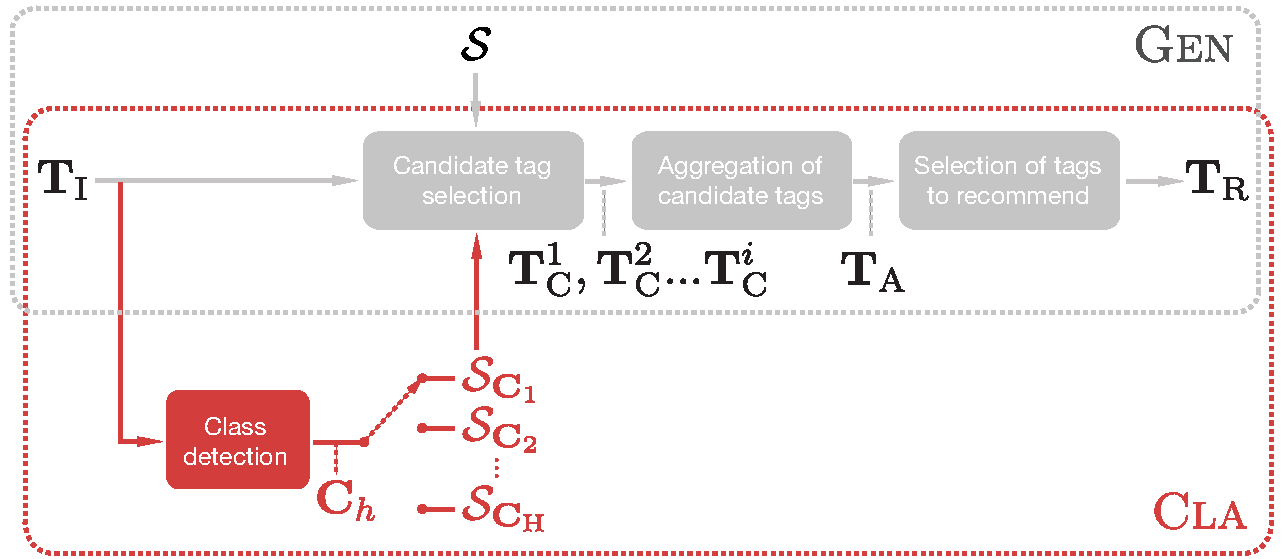
\includegraphics[width=1.0\columnwidth]{ch04_class/pics/fig_both_diagrams.pdf}
  \caption[Block diagram of the general and class-based tag recommendation methods]{Block diagram of the general (\textsc{Gen}) and class-based (\textsc{Cla}) tag recommendation methods.}
  \label{class:fig:diagrams}
\end{figure}

\begin{enumerate}
\item Candidate tag selection: Given a set of input tags $\inputTags$, this step uses a tag-tag similarity matrix $\similarityMatrix$ derived from the Freesound folksonomy to select a set of $\nCandidateTagsPerInputTag$ candidate tags $\candidateTagsPerInputTag$ for each input tag $\inputTag$. The tag-tag similarity matrix $\similarityMatrix$ is constructed by computing the association matrix $\associationMatrix = \left\{ \associationMatrixElement_{i,j} \right\}$, which represents the associations between tags and sounds in the Freesound folksonomy ($\associationMatrixElement_{i,j} = 1$ if sound $\audioClip_i$ is labeled with tag $\tagb_j$, and $\associationMatrixElement_{i,j} = 0$ otherwise). %Hence, $\associationMatrix$ is a sparse matrix that has as many columns as sounds in Freesound and as many rows as the set of distinct tags being used to label these sounds.%\footnote{In order to reduce the computational cost of the operations performed in this step and to get rid of potentially noisy tags, when building the association matrix we only consider tags whose frequency of occurrence is higher than a threshold $\tagFrequencyThreshold=10$ (i.e.,~we only consider tags that are used at least 10 times in the Freesound folksonomy). In this way the number of rows of the association matrix is reduced by $\approx$80\%, with only around $\approx$10\% of the associations between tags and sounds being actually ignored (Sec.~\ref{sec:general:datasets}).}. 
Given $\associationMatrix$, the tag-tag similarity matrix is obtained as $\similarityMatrix = \associationMatrixMultiplication'$, and we apply a simple normalisation to the elements $\left\{ \similarityMatrixElement_{\tagb_i,\tagb_j} \right\}$ of $\similarityMatrix$ so that $\similarityMatrixElement_{\tagb_i,\tagb_j}$ corresponds to the cosine similarity between tags $\tagb_i$ and $\tagb_j$ on the basis of their co-occurrence in sounds. Tags in $\candidateTagsPerInputTag$ are selected as the $\nCandidateTagsPerInputTag=100$ most similar tags to a given input tag $\inputTag$.

\item Aggregation of candidate tags: Given the sets $\candidateTagsPerInputTag$ from the first step, candidate tags are assigned a score $\scoreCandidateTag$ and aggregated into a single list of tags with scores $\aggregatedCandidateTags$. Such a score is determined by the candidate similarity-based ranking so that $\scoreCandidateTag=1$ for the most dissimilar candidate to a given input tag and $\scoreCandidateTag=\nCandidateTagsPerInputTag$ for the most similar one. The scores of tags that are present in different sets of candidates $\candidateTagsPerInputTag$ are added when aggregated in the final set $\aggregatedCandidateTags$.

\item Selection of tags to recommend: Considering the scores in $\aggregatedCandidateTags$, this step determines a threshold $\scoreThreshold$ to select the tags that are finally recommended. Here we use the strategy of determining the threshold $\scoreThreshold$ as a percentage of the maximum score in $\aggregatedCandidateTags$, and use a percentage parameter of $\percentageOfPercentageStrategy=0.15$ (Sec.~\ref{sec:general:percentage_strategy}). Tags in $\aggregatedCandidateTags$ are sorted by their score and those that satisfy $\scoreCandidateTag \geq \scoreThreshold$ are outputted as $\recommendedTags$, the final set of recommended tags.
\end{enumerate}

\subsection{Class-based tag recommendation}
\label{class:sec:class_based_tag_rec_ref}

The proposed class-based tag recommendation method is a variation of \textsc{Gen} based on the classification of the input tags $\inputTags$ into a set of $\nAudioClasses$ predefined audio classes\footnote{When referring to audio classes, we may use the terms ``class'' or ``category'' indistinctly.}. For every class $\audioClass$ ($\audioClass \in \audioClasses$, where $\audioClasses$ is the set of defined audio classes), a tag-tag similarity matrix $\similarityMatrixOfClassH$ is built in the same way as in the \textsc{Gen} method, except that in this case only the information of tag applications involving the sounds of the current class is considered (see below). As a result, a different tag-tag similarity matrix can be computed for every audio class, and the matrix $\similarityMatrixOfClassH$ that is used in the candidate tag selection step of the recommendation process depends on the classification of the input tags $\inputTags$ (Fig. \ref{class:fig:diagrams}).
Once the candidates are selected, the other two steps (Aggregation of candidate tags and Selection of tags to recommend) are computed in exactly the same way as in \textsc{Gen}.
We now describe the classification system that we use in the class detection step, and then explain the computation of the tag-tag similarity matrices.


\subsubsection{Classification system}
\label{class:sec:classification_system}

In order to classify a set of input tags $\inputTags$ of a sound $\resource$ into one of the audio classes, we make use of standard machine learning techniques. The structure of the classification system is very similar to what can be found in the existing literature on the classification of sound effects~\citep{Kuo1999,Casey2002,Sundaram2008,Roma2010}, musical instruments~\citep{Herrera2003,Livshin2003,Cano2004}, or music genre and mood~\citep{laurier2008,Bischoff2009,Chen2009,Tao2010}.
In these works, a set of low-level audio features is typically extracted from sounds in a given collection, yielding a feature vector representation of every sound. Also, sounds are manually annotated using the concepts of a taxonomy representing the particular classification domain (e.g.,~a taxonomy of musical instruments or sound effects). These taxonomies tend to be rather small, typically including less than 20 concepts. Then, supervised learning is performed using a classifier trained with the feature vectors corresponding to annotated sounds. 
%Some of these studies also make use of use of textual data such as lyrics and social tags at some point in the classification process but, to the best of our knowledge, no audio classification systems have been researched that only use information coming from tagging systems.

The classification we perform here only differs from this scheme in that we do not extract audio features from the sounds we classify, but use instead their existing associated tags (i.e.,~taglines) as feature vectors to train the classifier.
To do this, we follow a bag-of-words approach where each sound is represented as a vector whose elements indicate the presence or absence of a particular tag. 
Feature vectors contain all possible tags in the collection, thus their dimensionality is very high. 
Here we do not carry on any dimensionality reduction step to lower the size of the feature vectors. Instead, in order to keep them in manageable sizes, we apply the same threshold $\tagFrequencyThreshold=10$ described in Secs.~\ref{sec:general:datasets} and~\ref{class:sec:Gen}, removing all tags that are used less than 10 times.
The resulting feature vectors are very sparse, which makes the problem similar to what is normally found in text classification, where high dimensionality and sparseness are commonplace~\citep{Sebastiani2002}.
We experiment with a support vector machine (SVM) and a naive Bayes (NB) classifier, as these have been shown to be well suited for high dimensional and sparse classification tasks such as the one we are facing here~\citep{Bennett2000,Sebastiani2002}\footnote{We implement the classifiers using the  ``scikit-learn'' Python package (\url{http://scikit-learn.org}). We use the classes \texttt{LinearSVC} and \texttt{BernoulliNB} for SVM and NB, respectively, with default parameters. \texttt{LinearSVC} follows the ``one versus all'' approach for multiclass classification.}.
By not including extracted audio features in the classification system, we maintain a certain degree of generalisability for the class-based tag recommendation method, as the methodology remains applicable to other domains without further modifications. Nevertheless, what necessarily changes from domain to domain is the definition of classes.

\begin{table}
\ra{1.4}
\begin{center}
\footnotesize
\begin{tabular}{lp{9cm}}
\toprule
\multicolumn{1}{l}{\textbf{Class name}}	& \textbf{Description and examples} \\
\midrule
\textsc{SoundFX} & Sound effects (including \emph{foley}), footsteps, opening and closing doors, alarm sounds, cars passing by, animals and all kinds of noises or artificially created glitches.\\
\textsc{Soundscape} & Environmental recordings, street ambiances or artificially constructed complex soundscapes. \\
\textsc{Sample} & Instrument samples including single notes, chords and percussive hits (e.g.,~single notes of a piano recorded one by one and uploaded as different sounds, or samples from a complete drum set). \\
\textsc{Music} & Musical fragments such as melodies, chord progressions, and drum loops. This class is to \textsc{Sample} what \textsc{Soundscape} is to \textsc{SoundFX}. \\
\textsc{Voice} & Various voice-related sounds such as text reading, single words or recordings of text-to-speech processors. \\ 
\bottomrule
\end{tabular}
\end{center}
\caption[Name and descriptions of the audio classes]{Name and descriptions of the audio classes we defined.}
\label{tab:audio_classes}
\end{table}

Given the heterogeneity of the audio content in Freesound, we define the audio categories that we want to detect in a way that these can virtually include the whole range of sounds that can be found in Freesound.  
Hence, we define a total of $\nAudioClasses=5$ audio categories in which sounds can be classified. The resulting categories, shown in Table~\ref{tab:audio_classes}, are quite general and are in line with other sound categorisations reported in the literature~\citep{Casey2002, Roma2010}.
In order to create a dataset for the supervised learning process, we manually assigned one of the above categories to a number of sounds from Freesound. To do this, we followed an iterative process in which  we were presented with randomly chosen sounds from Freesound, and assigned them to one of the five categories. As it can be imagined, these categories are not completely orthogonal, and there were sounds for which the decision was not straightforward just by listening to the audio. In these cases, we also relied on provided textual descriptions of the sounds (i.e.,~their textual descriptions in Freesound). The crafted dataset includes a minimum of 2,088 sounds per category (corresponding to the case of \textsc{Speech}) and a maximum of 6,341 (for the case of \textsc{Samples}). Comparing the totality of Freesound sounds and the manually annotated subset, we observe qualitatively similar relative distributions of tag occurrences and number of tags per sound. 
Fig.~\ref{fig:tagclouds} shows the most commonly used tags for the five defined audio categories.
Using the manually crafted ground truth and the vector representations of sounds according to their taglines, we can train a classifier which, given a set of input tags $\inputTags$, can predict which category $\audioClass$ better fits the input.
In Sec.~\ref{class:sec:evaluation_classifier} we evaluate the classifier and report the results in terms of classification accuracy.

\begin{figure}
	\centering
		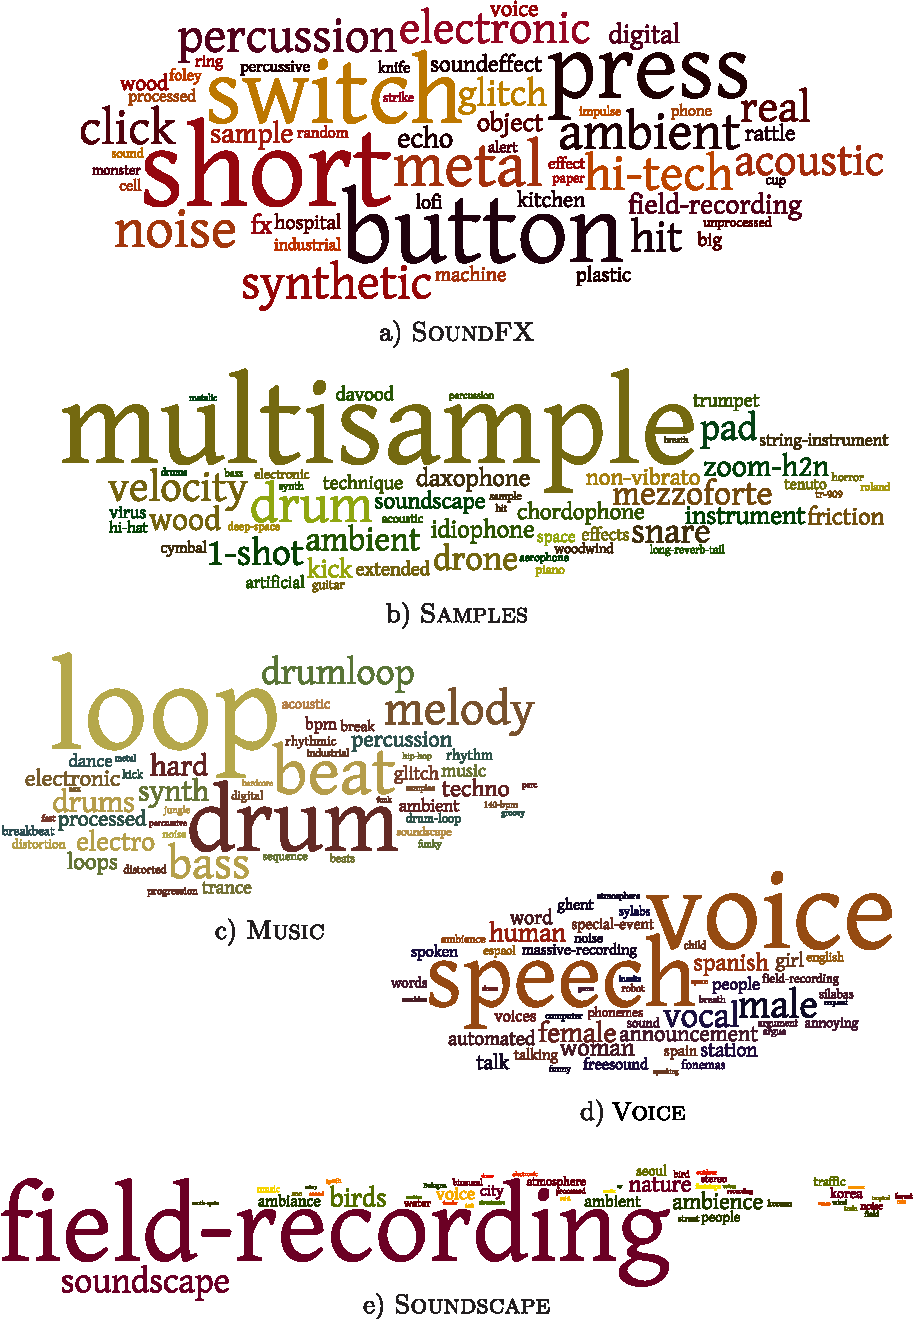
\includegraphics[width=0.95\columnwidth]{ch04_class/pics/tagclouds2.pdf}
	\caption[Tagclouds of the 50 most used tags in the five defined audio categories]{Tagclouds of the 50 most used tags in the five defined audio categories. The size of the tags is proportional to the frequency of occurrence among all sounds annotated under each category. For building these tagclouds, we only considered the set of sounds manually annotated as ground truth. Tagclouds were generated with the online tool available at \url{www.wordle.net}.}
	\label{fig:tagclouds}
\end{figure}


\subsubsection{Computation of tag-tag similarity matrices} 
\label{class:sec:similarity_matrix_computation}

As mentioned, the process of building the tag-tag similarity matrices $\similarityMatrixOfClassH$ is the same as the one for building $\similarityMatrix$, except that for every matrix $\similarityMatrixOfClassH$ we only consider information about tag applications from sounds belonging to $\audioClass$. 
For doing that, we reuse the classification system described above and classify all sounds of Freesound into one of the five audio classes, using as input tags the original taglines of the sounds in Freesound.  
Then, matrices $\similarityMatrixOfClassH$ can be built by only considering the columns of $\associationMatrix$ corresponding to the sounds of $\audioClass$. Hence, $\similarityMatrixOfClassH = \associationMatrixOfClassH\associationMatrixOfClassH'$, where $\associationMatrixOfClassH$ is a subset of $\associationMatrix$ in which the columns corresponding to sounds not in $\audioClass$ are removed.
Each matrix $\similarityMatrixOfClassH$ is normalised using the same process we use for $\similarityMatrix$ to obtain cosine similarity (Secs.~\ref{sec:general:step1} and~\ref{class:sec:Gen}). 

Notice that the similarity value between two tags $\tagb_i$ and $\tagb_j$ will be different in every matrix $\similarityMatrixOfClassH$ and in $\similarityMatrix$, with $\similarityMatrixOfClassH$ being tailored to the particular context of the $h$-th class. Note also that the number of distinct tags resulting from considering all sounds belonging to $\audioClass$ will be smaller than the total number of distinct tags resulting from considering all sounds from all classes (the size of the \emph{class vocabulary} will be smaller than the size of the \emph{general vocabulary}). Therefore, there will be some ``all-zeros'' rows in $\similarityMatrixOfClassH$, corresponding to the tags that are not used in the context of the particular class $\audioClass$. These tags are thus never recommended when using $\similarityMatrixOfClassH$.

\section[Results and evaluation of the classification system][Results and eval. of the classification system]{Results and evaluation of the classification system}
\label{class:sec:evaluation_classifier}

\subsection{Methodology}
\label{class:sec:evaluation_classifier_method}

To evaluate the classification system we follow a random sub-sampling cross-validation strategy where we split the aforementioned ground truth (i.e.,~the dataset) into training and testing sets. We then compute the out-of-sample accuracy as the percentage of well-classified instances from the testing set when using the fit from the training set. This process is repeated 100 times for each classifier and parameter configuration that we test (see below), and overall accuracy is obtained by averaging over the results of all repetitions. In each repetition, our dataset is composed of a random selection of 1,000 sounds from every category, adding up to a total of 5,000. This way we maintain a balance in the number of sounds per category. In addition, to avoid potential bias of our classifier to the tagging conventions of a particular user, we impose the limit of not getting more than 50 sounds of the same category uploaded by the same Freesound user. %We do that to avoid what could potentially be an equivalent of the \emph{album effect} that is known to happen in automatic music artist recognition~\citep{Whitman2001}. 
In each repetition, the testing set is selected as a random subset representing 10\% of the data, and being equally-distributed among categories (i.e.,~100 sounds per category). 

As mentioned in Sec.~\ref{class:sec:classification_system}, we test our method using SVM and NB classifiers. We also add a random classifier to serve as a baseline.
Given that for the class-based tag recommendation method the classification step is extensively used in situations with few input tags (i.e.,~when users start introducing tags), we are specially interested in evaluating the accuracy of the classification system in conditions of tag scarcity (i.e.,~low $|\inputTags|$).
Hence, we introduce a limitation to the testing set consisting of randomly removing tags from sounds prior to classification, only leaving a particular number of $N$ input tags per sound. We consider values of $N$ ranging from 1 to 5. This obviously adds another constraint to the selection of the testing set, which is to make sure that selected sounds have at least $N$ tags. The whole evaluation process is performed for all different values of $N$ and for both SVM and NB classifiers, yielding a total of 10 evaluated experiment combinations.

\subsection{Results}
\label{class:sec:evaluation_classifier_results}

\begin{figure}
	\centering
		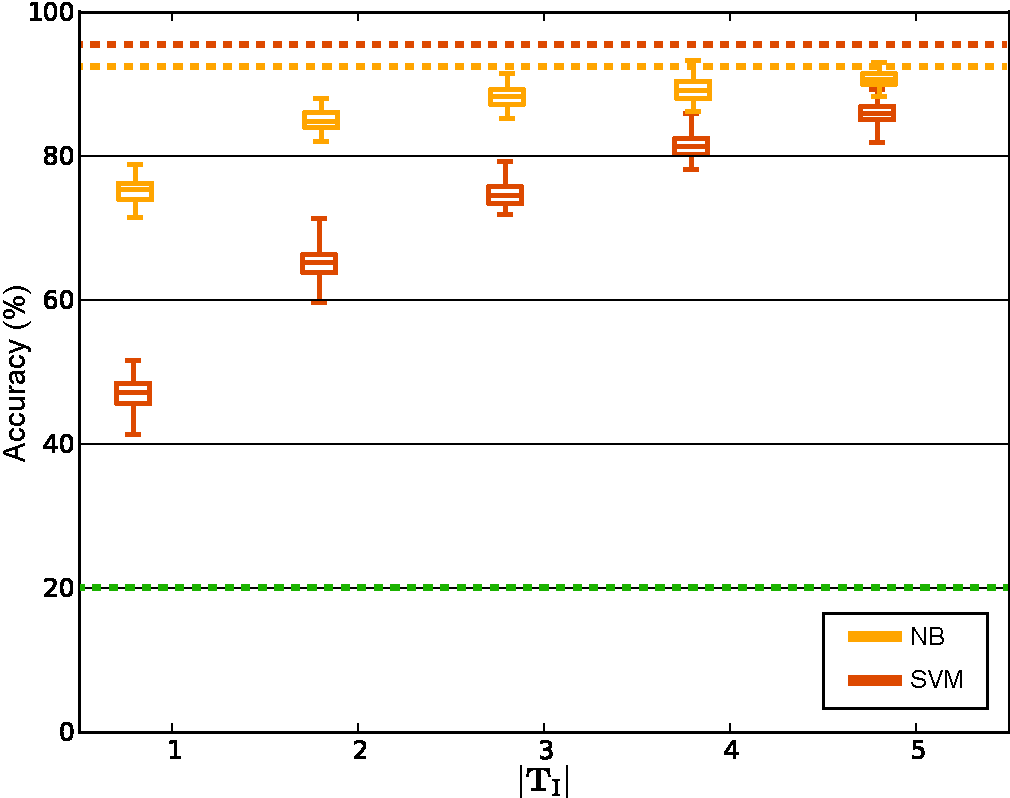
\includegraphics[width=\figSizeMid]{ch04_class/pics/classifier_results.pdf}
	\caption[Classification accuracy of the audio class detection step using SVM and NB classifiers]{Classification accuracy using SVM and NB classifiers. The dashed line at 20\% accuracy corresponds to the random baseline. The dashed lines around 95\% (SVM) and 90\% (NB) correspond to the accuracy achieved when no restriction on the number of tags for the testing set is performed, which can be considered as an upper bound limit.  
}
	\label{fig:classification_main_results}
\end{figure}

Fig.~\ref{fig:classification_main_results} shows the accuracies of our classification method for the experiment combinations described above. %(Sec.~\ref{class:sec:evaluation_classifier_method}). 
Note that all combinations are far above the random classifier accuracy of 20\%. The NB classifier reports overall a higher accuracy than the SVM, with a statistically significant average accuracy increase of 10\% ($p<10^{-12}$). Statistical significance is assessed by considering the maximum $p$-value across pairwise comparisons between experiment combinations and using the Wilcoxon signed-rank test with a significance level of 0.01~\citep{Corder2009}.
Overall, using the NB classifier, the classification system is able to successfully classify sounds among five generic categories inside the audio domain, with accuracies ranging from 75\% to 90\% depending on the number of input tags available for classification. 
As expected, the lowest accuracy is obtained when $|\inputTags| = 1$ (i.e.,~only one tag is given to the classifier). For $|\inputTags| \geq 4$, the classification accuracy reaches values close to 90\%. 

To complement these results, we performed additional experiments with different training set sizes (i.e.,~using less than than 90\% of sounds for training). The results we obtained are consistent with those reported above with little variation on accuracy for training set percentages higher than 50\%. This reinforces the validity of the classification results as the use of smaller training sets does not heavily affect classification accuracy. Furthermore, we also tested different values for the imposed maximum of 50 sounds uploaded by the same user in the same audio category. Our results show that the accuracy is not significantly influenced by such limit, thus asserting that the classifier is not biased to the tagging conventions of a particular user.% and questioning the existence of the aforementioned \textit{album effect} in our dataset. 
%\ref{class:sec:evaluation_classifier_method}


\section{Evaluation of the tag recommendation methods}
\label{class:sec:evaluation}

To evaluate the class-based tag recommendation method we designed an online experiment where participants had to tag a set of sounds from Freesound. 
The experiment was online for 15 days during June 2013, and was publicised in the Freesound front page. The goal of this experiment was twofold. 
First, we wanted to assess the usefulness of the \textsc{Cla} method with respect to the previous \textsc{Gen} method. 
Second, we wanted to get qualitative user feedback to better understand the strengths and weaknesses of the considered tag recommendation systems and, in a further stage, to understand the potential strengths and weaknesses of tag recommendation processes in general. 
%As mentioned in Sec.~\ref{sec:class:introduction}, this is yet an under-explored area.

Along with \textsc{Gen} and \textsc{Cla}, in the experiment we also evaluated two random variants of them, named \textsc{RGen} and \textsc{RCla}, respectively. These differ from the original variants in that, in the final step of the recommendation process, the set of recommended tags $\recommendedTags$ is replaced with an alternative set of the same length containing randomly selected tags either from the general vocabulary (\textsc{RGen}) or from the corresponding particular class vocabulary (\textsc{RCla}). Notice that the general vocabulary is always bigger than any of the individual classes' vocabulary. Hence, the random selection in \textsc{RGen} is performed over a bigger and more diverse pool of tags. Participants were not aware of the particular recommendation method underlying tag suggestions nor knew about the five audio classes in which we classify all annotated sounds. The dataset we used for the evaluation comprises Freesound data gathered between April 2005 and May 2012. % (Tables~\ref{tab:freesound_stats} and~\ref{tab:freesound_stats_sim_matrix}). 
Tables~\ref{tab:freesound_stats} and~\ref{tab:freesound_stats_sim_matrix} show basic statistics of the dataset and the resulting tag-tag similarity matrices that we built with this dataset.
%It includes tag applications which relate tags, sounds and users, and it is used to build the tag-tag similarity matrices $\similarityMatrix$ and $\similarityMatrixOfClassH$, as explained in Sec.~\ref{class:sec:similarity_matrix_computation}.
The online-experiment proceeded as follows:

\begin{table}
\begin{center}
\begin{threeparttable}
\ra{1.2}
\footnotesize
\begin{tabular}{p{8cm}r}
\toprule
\multicolumn{2}{c}{\textbf{Freesound dataset}} \\
\midrule
Number of sounds & 140,622  \\ 
Number of unique tags\tnote{a}  & 43,696  \\ 
Number of contributor users\tnote{b}  & 6,948  \\ 
Number of tag applications & 990,574  \\ 
Average tags per sound (tagline length) & 7.04  \\
\bottomrule
\end{tabular}
\begin{tablenotes}
    \item[a] Not necessarily semantically unique.
    \item[b] Users that have contributed by uploading, at least, one resource.
    \end{tablenotes}
  \caption[Basic statistics of the Freesound dataset]{Basic statistics of the Freesound dataset (including data collected between April 2005 and May 2012).}
\label{tab:freesound_stats}
\end{threeparttable}
\end{center}
\end{table}

\begin{table}
\ra{1.2}
\footnotesize
  \begin{center}
\begin{tabular}{lcc}
\toprule
\multicolumn{3}{c}{\textbf{Tag-tag similarity matrices}} \\  
& \textbf{Num. sounds} & \textbf{Vocabulary size} \\ 
\midrule

General matrix ($\similarityMatrix$) & 140,622 & 7,710 \\ 
Matrix for class \textsc{SoundFX} & 29,725 & 4,584 \\
Matrix for class \textsc{Soundscape} & 38,001 & 5,768 \\ 
Matrix for class \textsc{Sample} & 26,452 & 3,280 \\ 
Matrix for class \textsc{Music} & 34,139 & 4,303 \\ 
Matrix for class \textsc{Voice} & 15,305 & 3,557 \\
\bottomrule
\end{tabular}
  \caption[Basic statistics of the tag-tag similarity matrices]{Basic statistics of the resulting tag-tag similarity matrices.}
\label{tab:freesound_stats_sim_matrix}
  \end{center}
\end{table}


\begin{description}
  \item \textbf{Instructions page}: First, participants were presented with an introduction page displaying detailed instructions for the experiment (Fig.~\ref{class:fig:ss0_introduction}). Participants were told they would have to annotate 20 sounds from Freesound, using as many tags as they felt appropriate for every sound (we suggested participants to use five or more tags, but it was not mandatory). Participants were also told that as soon as they started typing tags, a list of tag suggestions would appear and that they could choose tags from this list if they felt the suggestions were appropriate. We also recommended participants to use headphones for better listening conditions.

\begin{figure}
  \centering
  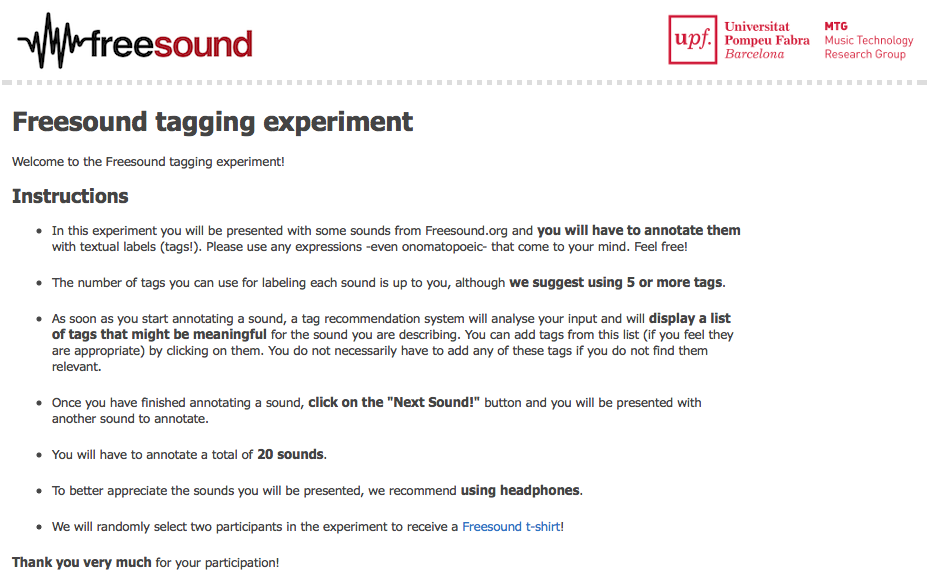
\includegraphics[width=1.0\columnwidth]{ch04_class/pics/fig_ss0_instructions.png}
  \caption[Screenshot of the instructions page]{Screenshot of the instructions page.}
  \label{class:fig:ss0_introduction}
\end{figure}

  \begin{figure}
  \centering
  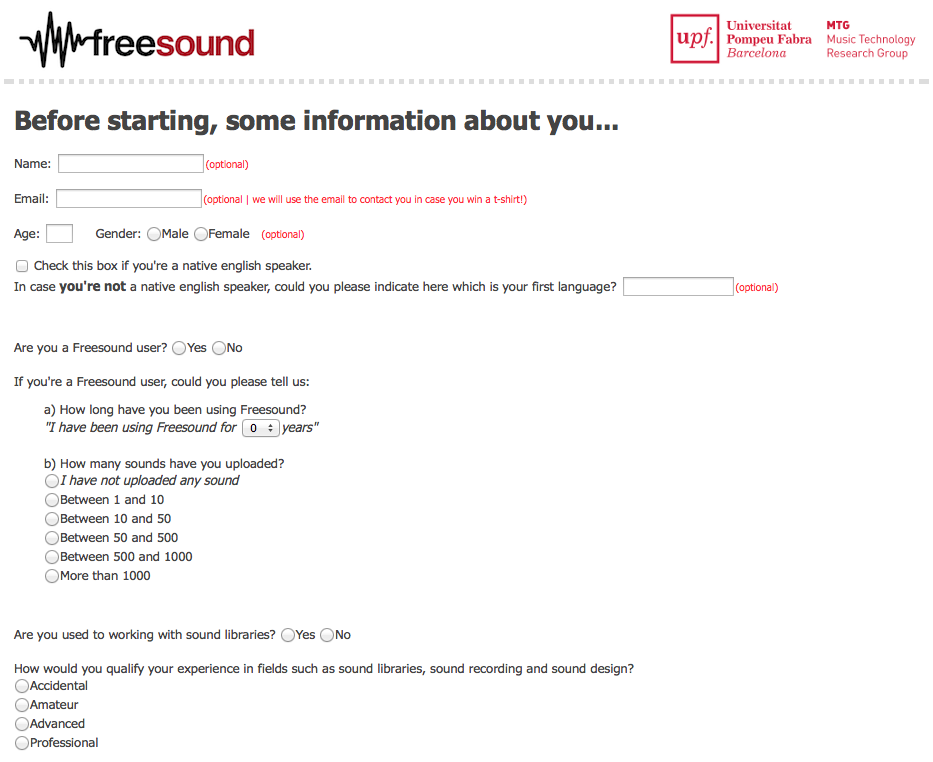
\includegraphics[width=1.0\columnwidth]{ch04_class/pics/fig_ss1_questionnaire.png}
  \caption[Screenshot of the questionnaire page]{Screenshot of the questionnaire page.}
  \label{class:fig:ss1_questionnaire}
\end{figure}

   \begin{figure}
  \centering
  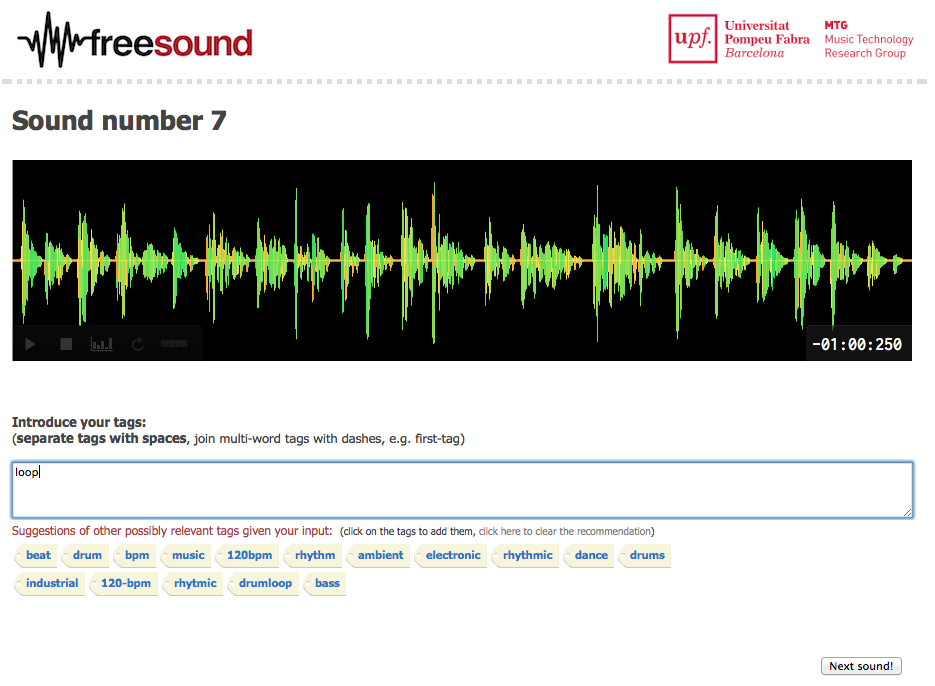
\includegraphics[width=1.0\columnwidth]{ch04_class/pics/fig_ss2_sound.png}
  \caption[Screenshot of the sound annotation page]{Screenshot of the sound annotation page.}
  \label{class:fig:ss2_sound}
\end{figure}

  \item \textbf{Questionnaire}: After the introduction, a short questionnaire (Fig.~\ref{class:fig:ss1_questionnaire}) was presented to collect some basic user data and information about their experience in working with sound libraries, their experience using Freesound (including the number of uploaded sounds) and their native language (in particular to be able to differentiate between native and non-native English speakers).

  \item \textbf{Sound annotation}: Once the questionnaire was completed, participants started annotating sounds. From the ground truth we defined when designing the recommendation system (Sec.~\ref{class:sec:classification_system}), we manually selected 50 sounds per class\footnote{The sounds we selected for the annotation phase of the online experiment (a total of 250, 50 per class) were removed from the ground truth and thus were not used to train the classifier described in section \ref{class:sec:classification_system}.}. These sounds were selected trying to cover a certain variety of sounds and avoiding those that would presumably be very hard to annotate. From this pool of 250 sounds, every participant was assigned a random selection of four sounds per class. Then, each of the four sounds was assigned a different tag recommendation method that would be used when the participant annotated the sound. In this way, every participant was assigned a total 20 sounds, equally distributed among audio classes and recommendation methods. Participants were presented with the first sound and had to annotate it by typing tags in a text box. The sound could be reproduced using a web player that also showed a visualisation of the waveform and the spectrogram of the sound (Fig.~\ref{class:fig:ss2_sound}). As soon as the participant started typing, a list of suggested tags appeared below the text box. This list was computed using the tag recommendation method assigned to the currently annotated sound, and was being updated every time a new tag was written in the text box. Similar to the Freesound upload system, tags had to be separated by spaces and multi-words joined with hyphens. Hence, the recommendation was primarily updated every time a blank space was introduced. Users could click over the tags shown in the list to automatically append them in the text box (Fig.~\ref{class:fig:ss2_sound}). Once a participant considered a sound was fully annotated, she could click on the ``Next sound'' button and be presented with the following sound. Participants were also provided an URL that they could save for later resuming the experiment in case they did not want to annotate all sounds in one go. Noticeably, we logged information about all the keystrokes and mouse clicks that participants performed with the corresponding timestamps.

  \item \textbf{Feedback page}: After annotating the 20 sounds, participants were presented with a page thanking their participation and offering some space in a text box to give some feedback about the experiment. Alternatively, they were also offered to write the feedback in a particular thread of the Freesound forums.

\end{description}

Considering the logs gathered during the experiment, we define a simple measure for evaluating the ``usefulness'' of every tag recommendation method in the tagging process. The measure consists of counting, for every set of tags assigned to a sound by a particular participant, the number of these tags that were recommended by the system during the annotation process (i.e.,~the number of recommended tags that were \emph{correctly predicted} by the system or, what is the same, \emph{accepted} by the participant). Then, this number can be averaged over all sounds annotated with each recommendation method, and obtain in this way a general characterisation of the method.
Let $\resources$ be a set of resources, let $\tagsOfSoundR$ be the set of tags that a participant used to annotate a particular sound $\resource$, and let $\nthRecommendedTagsInSession$ be one of the sets of recommended tags that were presented to the user in the successive $\numberOfTagRecommendationsInSession$ tag recommendations during the tagging process of that particular sound $\resource$. Then, we can define $\nAcceptedTags$, the number of correctly predicted tags (or accepted tags), as
\begin{equation}
\nAcceptedTags = \frac{1}{|\resources|} \sum\limits_{\resource\in \resources}{\left\vert \tagsOfSoundR \cap \left( \bigcup^{\numberOfTagRecommendationsInSession}_{\recommendationsInSessionIndex=1} \nthRecommendedTagsInSession \right) \right\vert} .
\label{class:eq:n_accepted_tags}
\end{equation}
Notice that $\nAcceptedTags$ is roughly equivalent to a standard recall measure (without the normalization term). We employ this measure instead of standard precision and recall (e.g.,~as done in~\citeauthor{Jaschke2009}~\citeyear{Jaschke2009}) because the nature of our evaluation has some particularities which make such metrics less useful. As described above, several tag recommendations are performed during the annotation of a single sound (i.e.,~every time that a new tag is introduced the recommendation is recomputed). As a result, the total number of recommended tags for every sound is much larger than the final number of assigned tags. If we computed precision and recall by comparing the whole set of recommended tags for every sound with the final taglines assigned by users, we would obtain very low precision values which, in our opinion, are not as representative as $\nAcceptedTags$. In our evaluation (and in a real-world tag recommendation scenario), users are the ones who finally decide which of the recommended tags are relevant for a particular resource. Therefore, the length of the recommendation is not as important as the fact that it contains meaningful suggestions (i.e.,~recall is arguably more important than precision).


\section{Results of the tag recommendation methods}
\label{class:sec:results}

During the two weeks the experiment was online, we gathered a total 201 experiment logs from 190 unique participants (a few participants decided to repeat the experiment more than once). Among all these experiment logs, 80 correspond to unfinished experiments (i.e.,~with less than 20 sounds annotated) which we do not consider in the analysis. In addition, we apply a filter to discard logs from experiments that were finished very quickly and with very few calls to the recommendation methods. More specifically, we discard logs from experiments completed in less than 10 minutes (average of 30 seconds per sound) and from experiments not reporting a minimum of three calls to the recommendation system for every annotated sound. We discard these logs as we consider that participants did not pay enough attention when annotating sounds and thus contain potentially noisy data. After filtering, we are left with 70 logs that we consider as sufficiently reliable data for analysis. In the following sections we report the results of the different aspects of the online experiment that we analyse.

\subsection{Correctly predicted tags per recommendation method}
\label{class:sec:accepted_tags_results}

First, we report the basic accuracy of the considered tag recommendation methods (Table~\ref{tab:results_general_ub}, leftmost column).
We observe that random methods \textsc{RCla} and \textsc{RGen} report considerably lower average $\nAcceptedTags$ than \textsc{Cla} and \textsc{Gen}. Thus, our methods generate much more meaningful recommendations than the random baselines. Interestingly, we also observe that both class-based methods \textsc{Cla} and \textsc{RCla} report higher averages than their general counterparts \textsc{Gen} and \textsc{RGen}. This suggests that tag recommendations improve when using class-based methods. However, the differences are found not to be statistically significant. In the following comparisons, and if not stated otherwise, statistical significance is assessed by performing pairwise comparisons using the Mann-Whitney U test with a significance level of 0.05~\citep{Corder2009}. 

\begin{table}
\ra{1.2}
\footnotesize
  \begin{center}
\footnotesize
\begin{tabular}{lc@{\hskip 0.65cm}cc@{\hskip 0.65cm}cc}
\toprule
	 %& \multicolumn{5}{c}{\textbf{Average number of correctly predicted tags}} \\
	 &  \textbf{All} & \textbf{Expert} & \textbf{Non-expert} & \textbf{Native} & \textbf{Non-native} \\ 
	 \midrule
 	\textsc{Cla} 	& 2.414 (2.775) 	&  2.547 (2.988) 	&  2.179 (2.224) 	&  2.950 (3.382) &  1.963 (2.027) \\ 
	\textsc{Gen} 	& 2.154 (2.526) 	&  2.163 (2.663)	&  2.147 (2.229) 	&  2.656 (3.006) &  1.732 (1.938) \\ 
	\textsc{RCla} 	& 0.260 (0.671) 	&  0.278 (0.680) 	&  0.211 (0.663) 	&  0.300 (0.705) &  0.226 (0.638) \\ 
	\textsc{RGen} 	& 0.166 (0.455) 	&  0.139 (0.458) 	&  0.253 (0.458) 	&  0.194 (0.518) &  0.142 (0.392) \\
	\bottomrule
\end{tabular}
\end{center}
\caption[Average number of correctly predicted tags per recommendation method]{Average number of correctly predicted tags $\nAcceptedTags$ (standard deviation in parenthesis) of the user-based evaluation approach for the different groups of participants.}
\label{tab:results_general_ub}
\end{table}

Next, we repeat the same analysis but considering different groups of experiment logs according to the questionnaire that participants had to fill at the beginning of the experiment (Table~\ref{tab:results_general_ub}). In particular, we compute $\nAcceptedTags$ for each recommendation method considering groups of logs corresponding to experienced participants (i.e.,~participants that checked the box marked with the question ``Are you used to working with sound libraries?'' in the questionnaire; second column in Table~\ref{tab:results_general_ub}), non-experienced participants (third column),  native English speakers (fourth column), and non-native speakers (fifth column). We again observe that \textsc{Cla} reports higher averages than \textsc{Gen}, which further supports the idea that class-based recommendations bring some improvements over the general method. Interestingly, in the case of experienced participants, the difference between \textsc{Cla} and \textsc{Gen} increases with respect to the same comparison when considering all participants. In this case we get a statistically significant increase of 0.38 ($\pvalue < 2.91\cdot 10^{-2}$). Furthermore, the difference between \textsc{RCla} and \textsc{RGen} also increases for the expert group (with respect to all participants) and becomes statistically significant ($\pvalue < 2.47\cdot 10^{-3}$). This suggests that expert participants clearly appreciate a difference between \textsc{Cla} and \textsc{Gen} methods (even for the random versions) and find class-based recommenders to be more useful. On the other hand, we observe that when analysing the non-experienced participants group, the differences between class-based and general methods gets blurred, with almost no difference between the two types of recommendation methods. Thus, non-experienced participants are not able to tell the difference between class-based and general recommendations. Overall, these results indicate that the usefulness of class-based tag recommendations compared to general recommendations is slightly higher, especially prominent in the case of experienced participants.

Considering the last two groups of participants (native and non-native English speakers), we observe that the differences between class-based and general recommendation systems are quite similar to those obtained when considering all participants. Class-based systems report higher $\nAcceptedTags$, but the increments are practically the same for both native and non-native groups (there is no statistically significant difference between the increments). Thus, we do not see a direct general implication of language in method preference. Nevertheless, there is a significant difference in the absolute number of correctly predicted tags among the native and non-native participant groups (Table~\ref{tab:results_general_ub}). Native English speakers tend to accept an average of 0.96 tags more than non-native ones ($\pvalue = 4.61\cdot 10^{-3}$). Furthermore, we observe that native English speaking participants tend to annotate sounds with an average of 0.32 tags more than non-native ones ($\pvalue = 3.24\cdot 10^{-6}$). This suggests that, in these experiments, native speakers use more tags for describing sounds than non-native speakers, and tend to accept more recommendations.  
%To the best of our knowledge, this is the first time evidence is reported with regard to the comparison of native's and non-native's tagging behaviour. 
%Our results suggest that native speakers use more tags when describing online resources than non-native participants. 
%Hence, this is an interesting aspect that should not be overlooked in future user-based evaluations and studies involving user participation. 
Overall, we see that both native and non-native speakers prefer \textsc{Cla} over \textsc{Gen} (and \textsc{RCla} over \textsc{RGen}), but that this preference is not stronger than in any of the other user groups.

\subsection{Correctly predicted tags per audio class}
\label{class:sec:accepted_tags_audio_class_results}

To gain insight into how recommendation methods work for the different audio classes defined above (Table~\ref{tab:audio_classes}), we group annotated sounds by their class and recommendation method, and computed the average number of correctly predicted tags $\nAcceptedTags$ for each group (Fig.~\ref{class:fig:accepted_tags_per_category_per_method}). In general, sounds under \textsc{Soundscape} and \textsc{Voice} classes report higher $\nAcceptedTags$ than sounds under the other classes. This is probably because there are some tags such as \texttt{field-recording}, \texttt{nature} or \texttt{voice} which are very common in these classes and are very generic (i.e.,~could be used to annotate almost any sound in \textsc{Soundscape} or \textsc{Voice} classes). 

\begin{figure}
  \centering
  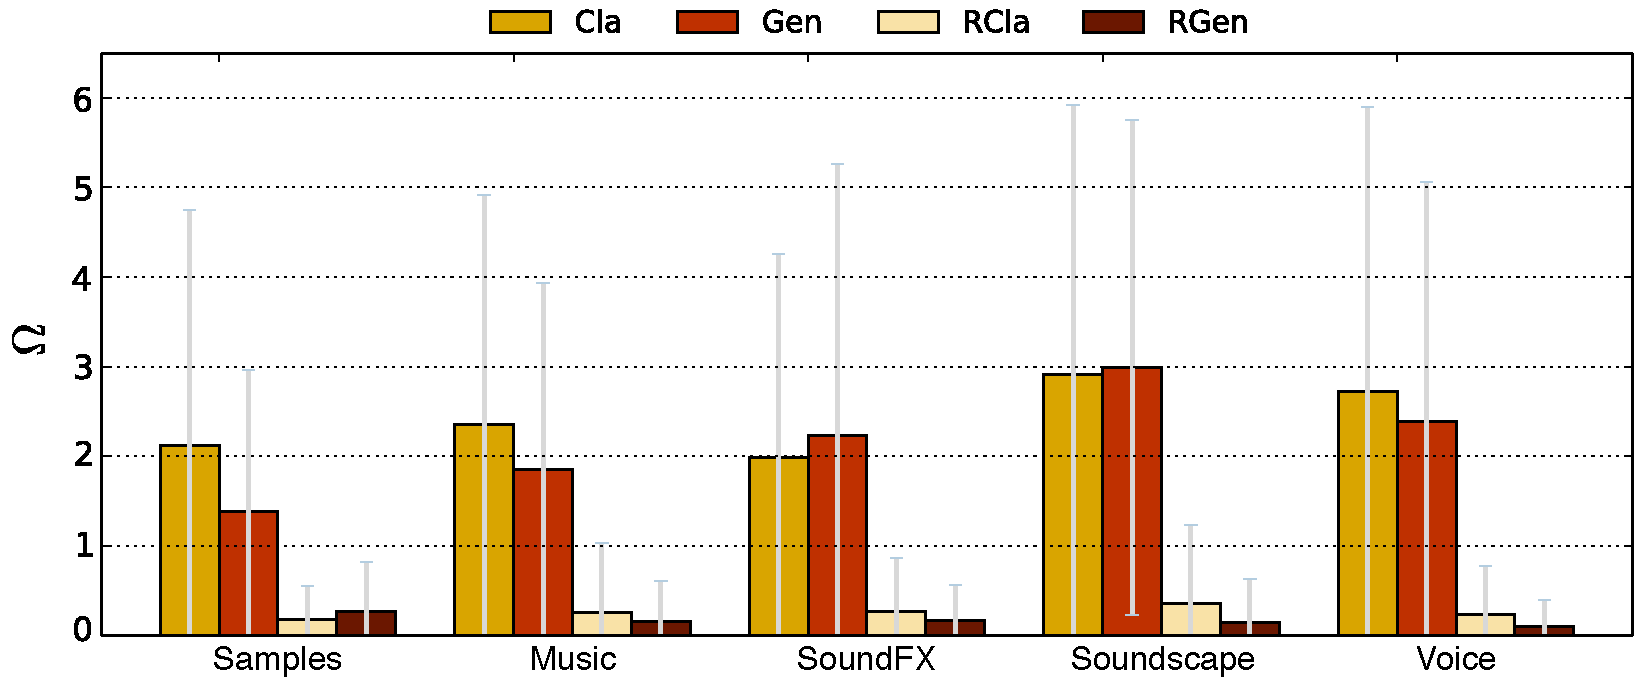
\includegraphics[width=0.85\textwidth]{ch04_class/pics/fig_AT_per_sound_category_per_method.pdf}
  \caption[Average number of correctly predicted tags per audio class and recommendation method]{Average number of correctly predicted tags $\nAcceptedTags$ per audio class and recommendation method.}
  \label{class:fig:accepted_tags_per_category_per_method}
\end{figure}

It can also be observed that not all audio classes feature higher $\nAcceptedTags$ for the \textsc{Cla} method when compared to the \textsc{Gen} method. \textsc{Soundscape} sounds report higher $\nAcceptedTags$ for \textsc{Gen} than for \textsc{Cla}, although the difference of 0.07 is not statistically significant ($\pvalue = 4.56\cdot 10^{-1}$). \textsc{SoundFX} sounds also report higher $\nAcceptedTags$ for the \textsc{Gen} method and, although the difference is still not statistically significant ($\pvalue = 3.80\cdot 10^{-1}$), the increase of 0.25 is this time larger. \textsc{Sample}, \textsc{Music} and \textsc{Voice} classes report higher $\nAcceptedTags$ for \textsc{Cla} recommendations, with larger $\nAcceptedTags$ increases and closer to statistical significance. This suggests that the adaptation to audio categories that the \textsc{Cla} method performs is better exploited in \textsc{Voice}, \textsc{Music} and \textsc{Sample} classes than in \textsc{Soundscape} or \textsc{SoundFX}. We hypothesise that the vocabulary needed to accurately describe sounds from the former classes is more reduced than the vocabulary needed for other sounds. 
Therefore, the class-based method can easily adapt to the class context and produce better recommendations.
These recommendations probably include tags which have a narrower semantic meaning than the tags recommended with the general method.
On the other hand, sounds under \textsc{Soundscape} and \textsc{SoundFX} classes cover a wider range of sounds and need a larger vocabulary to be well-described. In this situation, the \textsc{Cla} method does not adapt well and does not improve the  \textsc{Gen} results. Our hypothesis is partially supported by looking at the actual size of the resulting class vocabularies after computing the tag-tag similarity matrix per class ($\similarityMatrixOfClassH$, Table~\ref{tab:freesound_stats_sim_matrix}). \textsc{Voice}, \textsc{Music} and \textsc{Sample} produce smaller similarity matrices, with less tags in the vocabulary, than \textsc{Soundscape} and \textsc{SoundFX}.

\subsection{Correlation between number of uploaded sounds and the number of correctly predicted tags}
\label{class:sec:n_uploaded_sounds_at_correlation}

All participants in our experiment were Freesound users. However, not all of them had experience in uploading and tagging sounds in Freesound. In order to get some insight in how being used to tagging sounds affects $\nAcceptedTags$, we compute the correlation between the number of uploaded sounds and the number of accepted tags, grouping sounds into the four evaluated recommendation methods (Table~\ref{tab:correlation_uploaded_sounds_at}). To measure that correlation, we employ the Spearman's rank correlation coefficient~\citep{Corder2009}, with $\spearmanCorrelationCoefficient$ denoting the correlation coefficient and $\pvalue$ the $\pvalue$-value associated with it.

We find the strongest correlation for the \textsc{Cla} method ($\spearmanCorrelationCoefficient=0.276$, $\pvalue<3.76\cdot 10^{-7}$). Thus, in this case, $\nAcceptedTags$ tends to grow along with the number of uploaded sounds. A less significant correlation is reported for the \textsc{Gen} method ($\spearmanCorrelationCoefficient=0.105$, $\pvalue<5.61\cdot 10^{-3}$). \textsc{RCla} and \textsc{RGen} present no significant correlations ($\spearmanCorrelationCoefficient=0.087$, $\pvalue<1.13\cdot 10^{-1}$ and $\spearmanCorrelationCoefficient=0.063$, $\pvalue<2.55\cdot 10^{-1}$, respectively). This finding suggests that the more familiar the participants are with the Freesound uploading and tagging processes, the more recommended tags they tend to accept, especially when recommendations are generated with the \textsc{Cla} method. This result is consistent with the previous observation that experienced participants tend to accept more tags than non-experienced ones when recommendations are generated by \textsc{Cla} (Sec.~\ref{class:sec:accepted_tags_results}). Again, we are not aware of any study considering user familiarity in the context of resource tagging. Therefore, our results represent a novel and original contribution with regard to this aspect.
% the rank correlation coefficient was previously cited as hogg1995

\begin{table}
\ra{1.2}
\footnotesize
  \begin{center}
\footnotesize
\begin{tabular}{l@{\hskip 1.0cm}cccc}
	\toprule
	 %&  \multicolumn{4}{c}{\textbf{Average number of correctly predicted tags}}  \\
	 \textbf{Num. of uploaded sounds}	&  \textsc{Cla} & \textsc{Gen} & \textsc{RCla} & \textsc{RGem}  \\ 
	 \midrule
	  0 & 2.105 & 2.036 & 0.221 & 0.126 \\
	  1 to 10 & 1.823 & 2.027 & 0.293 & 0.133 \\
	  11 to 50 & 2.580 & 1.820 & 0.220 & 0.240 \\
	  51 to 500 & 2.289 & 2.222 & 0.311 & 0.133 \\
	  501 to 1000 & 4.160 & 2.035 & 0.380 & 0.300 \\ 
	  \bottomrule

\end{tabular}
\end{center}
\caption[Average number of correctly predicted tags per number of uploaded sounds and recommendation method]{Average number of correctly predicted tags $\nAcceptedTags$ per number of uploaded sounds and recommendation method. The ranges in the number of uploaded sounds are determined by the questionnaire that participants had to fill at the beginning of the experiment (Fig.~\ref{class:fig:ss1_questionnaire}).}
\label{tab:correlation_uploaded_sounds_at}
\end{table}


\subsection{Timing aspects}
\label{class:sec:timing_results}

Timing is also an often unconsidered aspect when evaluating tag recommendation systems. However, it is interesting because it can reveal some insights about the annotation process. In our experiments, we measured the average time invested for annotating a sound and observed that there exists a significant correlation between the length of the sounds and the time invested to annotate them, shorter sounds being the fastest to be annotated ($\spearmanCorrelationCoefficient=0.24$, $\pvalue<5.68\cdot 10^{-19}$). This could be expected, as shorter sounds tend to be less complex and need less time for listening to them. Consistently, sounds belonging to the \textsc{Soundscape} class need an average of 15 extra seconds to be described when compared to sounds belonging to other classes ($\pvalue< 8.12\cdot 10^{-3}$). On the other hand, \textsc{Sample} sounds need less time than the rest ($\pvalue < 3.15\cdot 10^{-2}$). This can be explained because \textsc{Soundscape} sounds are generally longer than sounds from other classes, while \textsc{Sample} sounds 
tend to be shorter. Nevertheless, when comparing the four different recommendation methods, we have not observed any statistically significant differences in the average time invested for annotating sounds. Therefore, in our particular comparison, the choice of a recommendation method does not seem to affect the time needed to annotate sounds.

\subsection{User feedback}
\label{class:sec:user_feedback}

In the last phase of the online experiment, participants were provided the opportunity to give some feedback in the form of textual comments (Sec.~\ref{class:sec:evaluation}). Looking at these comments, we observe some recurring opinions that,  if extrapolated, bring also valuable insights into recommendation processes in general. First of all, participants agree in that the process of annotating sounds (and by extension the process of recommending tags) is a very hard task, and that recommendations are a generally useful tool but not always needed or used. In fact, approximately 29\% of all tag annotations performed during the experiment were suggested by the recommendation systems\footnote{This percentage is computed without taking into account tag recommendations performed with random methods, which obviously did not provide meaningful recommendations.} (i.e.,~were correctly predicted), but the other tags were created by users.

A lot of participants point out that annotation is especially hard when the sound being described is not recorded/created by the person annotating it (which was always the case in our experiment). In these cases, there is a lot of meaningful information about the sound which most of the times can not be determined without the knowledge of how the sound was created (e.g.,~software used, recording device, location of a recording, etc.). Some participants also point out that in order to perfectly annotate musical sounds such as drum loops or instrument notes, a lot of time needs to be invested in determining properties such as beats per minute or the pitch of a note. These issues are particularly relevant in our context, where participants had to annotate sounds not created by themselves. Finally, another repeated comment is that tag suggestions are more useful for ``nature'' and ``human-related'' sounds, whereas ``abstract'' and ``synthetic'' sounds require more tags to be manually introduced 
before some meaningful suggestions are made. These comments are somehow aligned with the results reported in Fig.~\ref{class:fig:accepted_tags_per_category_per_method}, where we see that \textsc{Soundscape} and \textsc{Voice} classes are the ones that report higher $\nAcceptedTags$.


\subsection{Tag analysis}
\label{class:sec:tag_examples}

Here we have a closer look at the experiment logs in order to get some insight into the type of tags that are recommended and in which cases these are correctly predicted. We observe several interesting patterns that we believe also help comprehend in more detail tag recommendation processes in general. First of all, there are some tags which are recommended and accepted many times in the online experiment. These tags correspond to very generic concepts such as \texttt{field-recording}, \texttt{voice}, \texttt{electronic}, \texttt{loop}, \texttt{nature} or \texttt{percussion}. These recommendations are useful in providing some kind of general categorization to annotated sounds, but sounds only tagged with these kind of tags do clearly lack specificity in the annotations. We observe that another recommendation pattern consists of tags that are suggested many times but are rarely accepted. This is the case of tags such as \texttt{sound} or \texttt{recording}, for which we hypothesise that the meaning is too obvious to be considered as relevant information for participants. This is also the case of tags like \texttt{soundscape}, \texttt{percussion-loop}, \texttt{drum-loop} or \texttt{natural-reverb}, which can typically be represented with alternative tags, compound-tags or pairs of tags such as \texttt{field-recording} (instead of \texttt{soundscape}), \texttt{loop}, \texttt{percussion}, \texttt{drum}, \texttt{natural} or \texttt{reverb}.

We also observe that there are some tags whose low acceptance can be explained because of its subjective meaning (e.g.,~\texttt{groovy}, \texttt{threatening}) or because participants can not assess its correctness because they are not the authors of the annotated sounds (e.g.,~\texttt{multi-sample}, \texttt{improvised}). Obviously there are also some suggested tags which are not accepted because they are simply not appropriate for the sounds being described. This is the case of tags like \texttt{piano}, \texttt{guitar} or \texttt{pad}, which are sometimes recommended to sounds that clearly do not contain piano, guitar or pad-like sounds. Finally, we observe a last group of suggestions which correspond to tags not usually suggested but normally accepted such as \texttt{annoucement}, \texttt{syn\-the\-sizer}, \texttt{footsteps} or \texttt{airplane}. We consider these as being very good recommendations as they correspond to not-so-general concepts and are apparently recommended only when they are needed. Overall, recommendations provided by our methods tend to be useful when recommending general tags, referring to concepts that can be used as a broad categorisations of the sounds. However, recommendations are not as useful when they refer to more detailed aspects of the sounds being annotated.


\section[Complementary results and evaluation of the tag recommendation methods][Comp. res. and eval. of the tag rec. methods]{Complementary results and evaluation of the tag recommendation methods}
\label{class:sec:pb_evaluation}

In order to complement the user-based evaluation, we also consider a systematic assessment of the different tag recommendation methods (\textsc{Cla}, \textsc{Gen}, \textsc{RCla} and \textsc{RGen}) following the methodology we described in Chapter~\ref{sec:general}. This complementary assessment follows a setup based on a tag prediction task which we now describe.

\subsection{Methodology}

For this evaluation we consider sounds and annotations of the same Freesound dataset described in Sec.~\ref{class:sec:evaluation}. 
The process we follow is very similar to that described in Chapter~\ref{sec:general} (Sec.~\ref{sec:general:evaluation_methodology_a}).
However, for each fold of the 10-fold cross-validation, we now have to follow two extra steps to set up the system for producing tag recommendations.
The first step consists of training a classifier that allows the classification of the input tags into one of the five defined audio classes. We train the classifier as described in Sec.~\ref{class:sec:classification_system}, but feeding the classifier only with these sounds that are present both in the training set of the current fold and in the ground truth we built when designing the system (i.e.,~we only use sounds from the training set that we know to which audio category they belong to).

The second step of the training phase consists of building the general tag-tag similarity matrix $\similarityMatrix$ and the matrices $\similarityMatrixOfClassH$ for every class $\audioClass$. For this we use information from all the sounds in the training set. Notice that building $\similarityMatrixOfClassH$ requires the classification of all sounds of the training set into one of the five defined categories (Sec.~\ref{class:sec:similarity_matrix_computation}). We perform that classification using the same classifier trained in the first step of the training phase. Hence, this classifier is not only used during the recommendation process to automatically detect the audio class of a set of input tags $\inputTags$, but it is also used to build the different tag-tag similarity-matrices $\similarityMatrixOfClassH$ corresponding to each audio class.

Similarly to Sec.~\ref{class:sec:classification_system}, after the training phase we pick every sound in the evaluation set and randomly delete a set of tags $\deletedTags$ from its originally assigned tags, yielding $\inputTags$, the input to our recommendation system. The number of tags we delete is chosen uniformly at random, with only the constraint of leaving a minimum number of input tags of $|\inputTags| \geq 3$ so that there is presumably enough information for the recommender systems to provide good recommendations (see Sec.~\ref{sec:general:datasets}). This constraint also implies that, in order to be able to remove at least one tag for each sound ($|\deletedTags| \geq 1$), we can only consider for evaluation the sounds that have at least four tags\footnote{This filtering is done before the whole evaluation process starts, therefore we evaluate the same number of sounds in each fold.}. After we remove some tags, we run the four tag recommendation methods using $\inputTags$ as input and the similarity matrices we computed in the training phase. 
%As evaluation measures we compute standard precision ($\precision_\audioClipEvaluatedInComplementaryEvaluation$), recall ($\recall_\audioClipEvaluatedInComplementaryEvaluation$), and f-measure ($\fmeasure_\audioClipEvaluatedInComplementaryEvaluation$) for each individual sound $\audioClipEvaluatedInComplementaryEvaluation$ according to
As evaluation measures we compute standard precision, recall, and f-measure ($\precision$, $\recall$, and $\fmeasure$, respectively) for each evaluated sound (Eq.~\ref{eq:prf_ch2}).
%\begin{equation*}
%\precision_\audioClipEvaluatedInComplementaryEvaluation = \frac{|\recommendedTags \cap \deletedTags|}{|\recommendedTags|} \text{ }, \text{ }
%\recall_\audioClipEvaluatedInComplementaryEvaluation = \frac{|\recommendedTags \cap \deletedTags|}{|\deletedTags|} \text{ }, \text{ and }
%\fmeasure_\audioClipEvaluatedInComplementaryEvaluation = \frac{2 \precision_\audioClipEvaluatedInComplementaryEvaluation \recall_\audioClipEvaluatedInComplementaryEvaluation}{\precision_\audioClipEvaluatedInComplementaryEvaluation + \recall_\audioClipEvaluatedInComplementaryEvaluation},
%\end{equation*}
%where $\recommendedTags$ is the set of recommended tags and $\deletedTags$ is the set of deleted tags. 
Global $\precision$, $\recall$ and $\fmeasure$ measures for each tag recommendation method are calculated by averaging precision, recall and f-measure across all sounds evaluated with the chosen recommendation method.
Because of the nature of the tag prediction task, and as mentioned in Secs.~\ref{sec:soa:evluation_of_tag_recommendation},~\ref{sec:general:evaluation_methodology_a} and~\ref{general:sec:discussion}, tag recommendations in this evaluation are only considered as being ``correct'' recommendations if they contain tags originally assigned by the authors of the sounds. As a result, tags that could be subjectively considered as good recommendations for a particular sound but are not present in the original annotations do not count as correct predictions. Hence, the results provided by this evaluation are considered to be an underestimate of the real performance of the system.

%The prediction-based evaluation approach is interesting as it allows us to evaluate the different recommendation methods in a systematic way and using a lot of sounds. In the previous chapter, we used this evaluation methodology to exhaustively compare eight variations of the \textsc{Gen} recommendation method (using different sets of parameters for each one of the recommendation steps) against four baselines and two state of the art folksonomy-based tag recommendation methods, and using data from the folksonomies of Freesound and Flickr. 
%That number of methods could have not been comprehensively compared through a user-based evaluation approach such as the one presented in this chapter. However, prediction-based evaluation has an important limitation which is that we need an extensive ground truth to evaluate whether our predictions are correct or not. In our case, this ground truth is composed by the original taglines of sounds in Freesound. This means that the recommendations we evaluate will only be considered as ``correct'' recommendations if they contain tags that the original author of the sound used to annotate it. As a result, tags that could be subjectively considered as good recommendations for a particular sound but are not present in the original annotations do not count as correct predictions (see Secs.~\ref{sec:general:evaluation_methodology_a} and ~\ref{general:sec:discussion}). Moreover, prediction-based evaluation does not allow the collection of qualitative user feedback that, as we have seen before, can shed some light on relevant aspects of the recommendation process. For that reason, we state that the prediction-based evaluation approach may be taken as a complement to the results already described in the previous sections, allowing us to further test our previous findings.


\subsection{Results}

Results for the four evaluated tag recommendation methods (Table~\ref{tab:results_general_pb}) are very similar to those observed in the user study (Table~\ref{tab:results_general_ub}). We can see that \textsc{Cla} outperforms \textsc{Gen} by a small but statistically significant difference of 0.011 ($\pvalue < 6.51\cdot 10^{-8}$). This difference suggests that \textsc{Cla} can successfully take advantage of the classification step and the knowledge derived from the ground truth to slightly improve the recommendations of the system. As expected, random methods \textsc{RCla} and \textsc{RGen} score much lower $\fmeasure$ than \textsc{Cla} and \textsc{Gen}. Nevertheless, it is interesting to note that \textsc{RCla} also features a statistically significant increase in $\fmeasure$ with respect to \textsc{RGen} ($\pvalue < 1.57\cdot 10^{-24}$). This increase can be explained by recalling that the pool of tags from which the random selection is performed in \textsc{RCla} is different in every audio class and it always contains fewer tags than the pool in \textsc{RGen} (Sec.~\ref{class:sec:similarity_matrix_computation}). Hence, these results suggest that at least some tags which are not relevant for a particular audio class are effectively removed when building the similarity matrices $\similarityMatrixOfClassH$. We also observe that \textsc{Cla} and \textsc{Gen} feature a very similar number of recommended tags $\vert \recommendedTags \vert$, with an average of 3.99 and 3.88 tags, respectively.

\begin{table}
\ra{1.2}
\begin{center}
\footnotesize
\begin{tabular}{l@{\hskip 1cm}cccc}
\toprule
	  \textbf{Method} & \textbf{Precision} & \textbf{Recall} & \textbf{F-measure} \\ 
	  \midrule
	\textsc{Cla}  & 0.476 (0.428) 		&  0.488 (0.424) 		&  0.440 (0.389) \\ 
	\textsc{Gen}  & 0.486 (0.429) 		&  0.467 (0.408) 		&  0.429 (0.372) \\ 
	\textsc{RCla} & 0.003 (0.031) 		&  0.003 (0.038) 		&  0.002 (0.025) \\ 
	\textsc{RGen} & 0.002 (0.024) 		&  0.002 (0.031) 		&  0.001 (0.019) \\ 
\bottomrule
\end{tabular}
\end{center}
\caption[Average precision, recall and f-measure per recommendation method]{Average precision $\precision$, recall $\recall$ and f-measure $\fmeasure$ (standard deviation in parenthesis) for the prediction-based evaluation approach. Results are sorted by f-measure.}
\label{tab:results_general_pb}
\end{table}

If we analyse $\fmeasure$ as a function of the number of input tags $|\inputTags|$ and the number of recommended tags $|\recommendedTags|$, we can get more insight on the behaviour of the considered recommendation methods (Fig.~\ref{class:fig:f_measure_pb_evaluation}). For instance, we see that both \textsc{Cla} and \textsc{Gen} have a tendency of increasing $\fmeasure$ as the number of input tags also increases (Fig.~\ref{class:fig:f_measure_pb_evaluation}a).
Note that, as we have seen in Sec.~\ref{class:sec:evaluation_classifier_results}, the accuracy of the classifier also increases for larger $|\inputTags|$, which is consistent with these results.
Overall, we see that the recommendation system is able to provide better recommendations when it is fed with more input tags. The opposite happens with the number of recommended tags (Fig.~\ref{class:fig:f_measure_pb_evaluation}b). This can be explained as bigger numbers of recommended tags imply lower precision values because more non-relevant tags are recommended. Nevertheless, it is interesting to observe that the increase in $\fmeasure$ of \textsc{Cla} over \textsc{Gen} is specially notorious for large numbers of recommended tags ($\vert \recommendedTags \vert > 8$, Fig.~\ref{class:fig:f_measure_pb_evaluation}b). 
This highlights the superiority of \textsc{Cla} over \textsc{Gen} when larger number of tags are recommended, and suggests that \textsc{Cla} is able to provide more comprehensive and relevant recommendations.

\begin{figure}
  \centering
      \subbottom[]{
      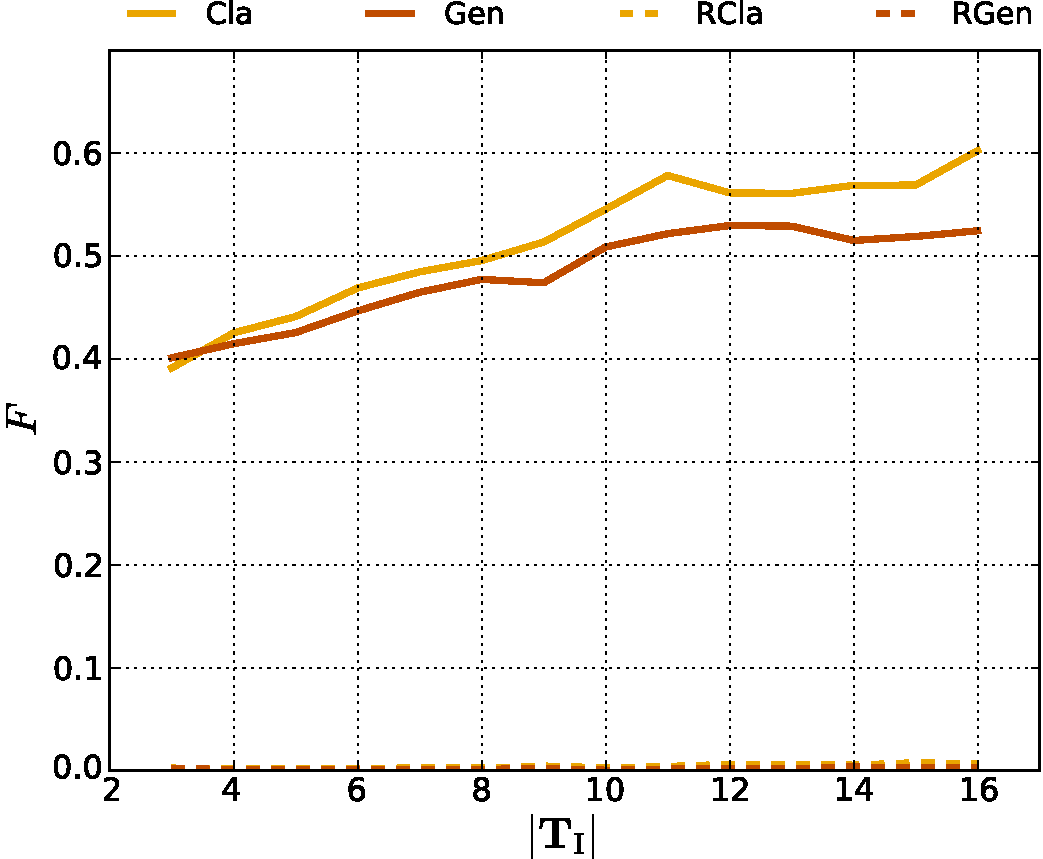
\includegraphics[width=\figSizeMid] {ch04_class/pics/fig_pb_evaluation_f_vs_input_tags.pdf}
      }
      \subbottom[]{
	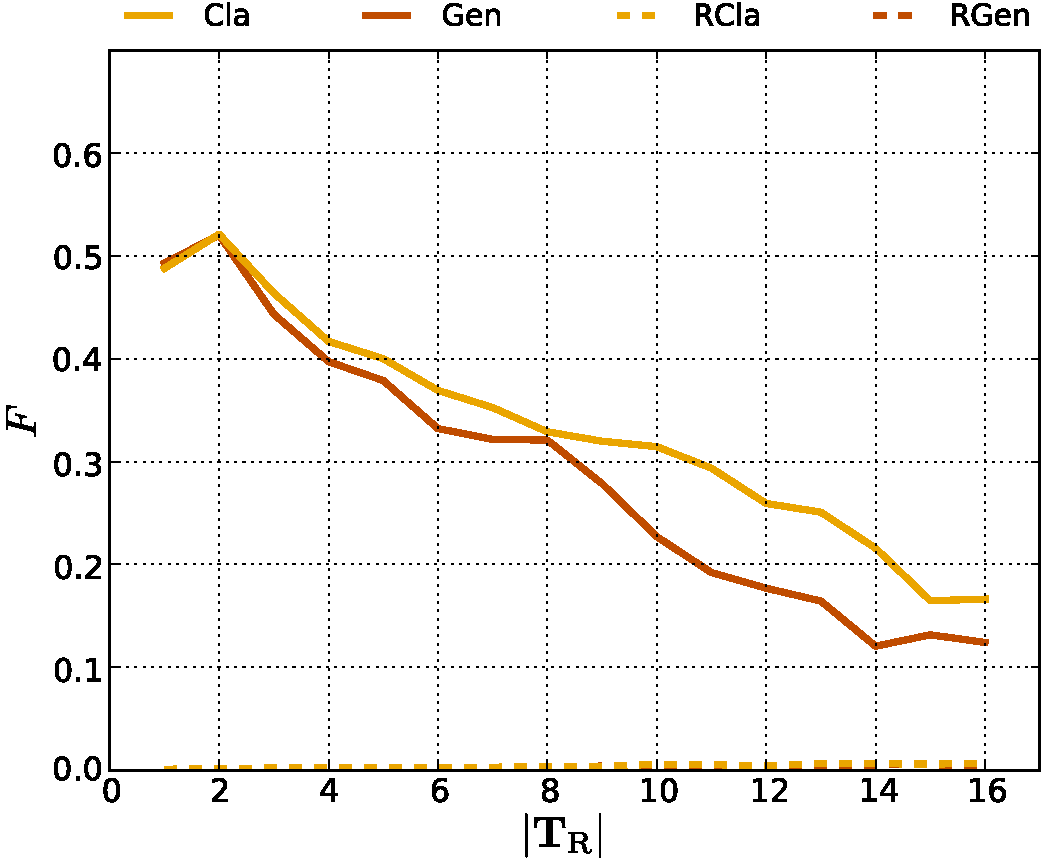
\includegraphics[width=\figSizeMid] {ch04_class/pics/fig_pb_evaluation_f_vs_added_tags.pdf}
      }
     \caption[Average f-measure as a function of the number of input tags and the number of recommended tags]{Average f-measure $\fmeasure$ as a function of the number of input tags $|\inputTags|$ (a) and the number of recommended tags $|\recommendedTags|$ (b).}
  \label{class:fig:f_measure_pb_evaluation}
\end{figure}


\section{Conclusion and discussion}
\label{class:sec:discussion}

In this chapter we have described an extension of the best performing tag recommendation method described in Chapter~\ref{sec:general}, and thoroughly evaluated it.
The method we described here extends the former in two main aspects: it automatically determines to which class a sound belongs, and it produces specific recommendations for different audio classes. 
As both tag recommendation methods (\textsc{Gen} and \textsc{Cla}) are folksonomy-based, they are easily generalisable to other multimedia domains. However, the \textsc{Cla} method requires the definition of a number of classes of resources in the particular domain, and the construction of a ground truth to train the classifier needed to perform recommendations. 

%The main bottleneck in terms of scalability lies in the computation of the tag-tag similarity matrices that inform the candidate selection step. However, these matrices can be computed offline, and their size can be easily reduced by raising the threshold $\tagFrequencyThreshold$ during the construction of the association matrix. This will discard those tags whose frequency of occurrence is below that threshold (Sec.~\ref{class:sec:Gen}). That means that our recommendation methods can scale well to even bigger amounts of data, as the number of tags above the threshold $\tagFrequencyThreshold$ will grow much more slowly than the number of resources.

%A limitation of the proposed recommendation methods is that they can suffer the \emph{cold-start} problem if deployed to collaborative tagging systems which have not enough data to derive reliable tag-tag similarity matrices. 
%Although our recommendation methods have not been designed for collaborative tagging systems with scarce data, it would be interesting to evaluate how fast the methods could acquire enough data from user annotations in order to provide meaningful recommendations. 
%In other words, it would be interesting to investigate how big the folksonomy of a collaborative tagging system should be to enable our tag recommendation methods to provide meaningful recommendations. 
%We hypothesise that, on a first step of the implementation of the system, tag-tag similarity matrices would need to be recomputed very often as relatively small changes in the folksonomy could have a big impact on the resulting similarity matrix. In that case, the system would quickly learn from user tagging behaviour and recommendations would quickly start to become more diverse. Besides the similarity matrices, the \textsc{Cla} method also needs annotation data to train the classifier. However, a collaborative tagging system could start using the \textsc{Gen} method until enough data would be collected to build the ground truth and train the classifier.

We performed a user-based evaluation through an online experiment. In it, participants had to annotate several sounds with the help of the different tag recommendation strategies. We logged the activity of the participants and analysed these logs with the goal of comparing the considered methods and, in addition, getting more insight into the positive and negative aspects of tag recommendation systems in general. To the best of our knowledge, this is one of the very few user-based evaluations carried out for a tag recommendation task. Finally, as a further contribution, we complement the user-based evaluation with a prediction-based evaluation, following a well-established methodology.

In general, we have seen that class-based recommendation reports statistically significantly better scores than general recommendation, both in the user-based and prediction-based evaluations. The difference in scoring is, in absolute terms, more prominent for the user-based evaluation. Moreover, it further improves when considering only expert users. This suggests that the class-based method does indeed bring some improvements in the recommendations compared to the general method, and that these improvements are more noticeable to expert users.

Among all annotations that participants performed during the online experiment, approximately one third of them correspond to tags recommended by the system (for both \textsc{Gen} and \textsc{Cla} methods). That by itself brings evidence with regard to the general utility of tag recommendation systems. However, the found results also indicate that tag suggestions referring to generic concepts or sound classes tend to be more useful than recommendations of very concrete tags describing specific sound characteristics. Participants found tag suggestions more useful for sounds under \textsc{Soundscape} and \textsc{Voice} categories. We hypothesise that this happens because these categories are more suited to the use of generic tags. \textsc{Music} and \textsc{Sample} audio classes require of annotations describing very specific musical concepts such as pitch, tonality or beats per minute. Participants had difficulties in annotating such concepts, as they are problematic to annotate without having a certain knowledge of the recording context (i.e.,~without being the author of the sound) and because tag recommenders tend to produce less meaningful suggestions in these cases. %All these often overlooked qualitative evaluation aspects also represent a valuable contribution of the present article.

Summarising, here we continued with the research described in the previous chapter by proposing an extended tag recommendation method that incorporates basic knowledge of the audio domain, and by comparing, with an online experiment, the extended method with the best scoring method of the previous tag recommendation scheme.
In the next chapter (Chapter~\ref{sec:impact}), we further investigate on tag recommendation by analysing the impact of the class-based method in a large-scale experiment on the real-world tagging system of Freesound.


% I REMOVED THIS BIT AS WE ALREADY COMNMENT ON THAT AT THE CONCLUSION OF THE NEXT CHAPTER
%Leaving aside the potential impact of tag recommendation in a real-world tagging system, we believe that in order to build better tag recommendation systems, those must be more aware of the particular contexts of the resources being described and must extensively exploit all available knowledge. To generate tag suggestions describing more concrete aspects of sound characteristics we need systems that know about the specifics of the audio domain, such as which are the most relevant properties of sounds for different audio categories, and how to automatically estimate some of these properties. In Chapter~\ref{sec:ontology}, we explore this perspective by proposing an extension of the tag recommendation method described here which takes advantage of a domain-specific ontology to drive the recommendation process.


%For that reason, we believe that future tag recommenders should take advantage of knowledge representation mechanisms such as ontologies to be able to include tags describing the audio domain in some structured representation, and to be able to produce informed recommendations based on reasoning and users' input. Such a system should contribute in greatly improving online resource descriptions and thus facilitating and providing new opportunities for content reuse.

% We have not investigated the use of more precise categories as our current goal is the classification of audio sounds in Freesound in broad categories that allow further tailored treatment, and not the classification of these audio sounds into a more specific taxonomy that could be used as an interface for browsing Freesound content. 

% We have also defined such categories so that they can, in a near future, allow us to apply meaningful different treatments tailored to different types of audio sounds